
\chapter{Aspects neurophysiologique: son, écoute}


\section{Le son}

Lors d'un concert, si nous pouvions visualiser les sons qui
s'échappent de l'orchestre, ce serait un chatoiement de cercles qui se
répandraient tout autour de nous, comme 
la propagation des
ronds dans l'eau suite à un ébranlement de sa surface.
Les molécules d'air en contact avec la source sonore se déplacent et
créent une vibration. \autocite[p. 183]{bencivelli:pourquoi,}.


Le son peut être déterminé par différents paramètres
physiologiques et psychologiques.
Il est défini très précisément par un ensemble d'unités physiques chiffrées
: les décibels  et les hertz.\footnote{Voir Annexe: Le son et sa
  définition.}




\section{Ecoute, perception des sons et troubles associés}
\paragraph{Ecouter ou entendre : une différence}

La définition du verbe `entendre' et du verbe `écouter' 
\autocite[pp. 361--385]{hachette:dictionnaire} nous paraît opportune
en raison de la confusion courante des deux termes :
\begin{description}
\item[Entendre] c'est  percevoir des sons, saisir par l'ouïe.
\item[Ecouter] a trois sens: 
\begin{enumerate}
	\item prêter l'oreille à; s'appliquer à entendre;
	\item prêter attention à l'avis de quelqu'un, suivre un avis;
	\item \emph{fig} suivre une impulsion,	une inspiration.
\end{enumerate}
\end{description}


En recherchant les sources étymologiques du
terme `écouter' , nous découvrons que 
 sa racine sanskrite \emph{ ``avih'' } se traduit par
 \emph{``évidence'' , ``connaissance'', ``discernement''}. Puis, en ancien
 français, ce mot a donné \textit{``oüir''} qui signifie aussi bien \textit{``entendre''} ,
\textbf{`` écouter'' } que \textit{``comprendre''}.\footnote{selon le dictionnaire d'étymologie et le site
  ``Etymologie Français latin grec Sanskrit-Google Sites'' }.
 Est-ce la raison
pour laquelle il subsiste toujours un amalgame 
sur le sens de ce verbe?
Selon Didier
Colin \footnote{Didier Colin,2015 ``Interprétez vos rêves''}, cette faculté
permet non seulement d'écouter et de comprendre avec plus d'attention
mais aussi de percevoir des sons et peut-être même, être doué de
\textit{``clairaudience'}'. 


En définitive, \emph{entendre} est une attitude passive par rapport au monde sonore
qui nous entoure. Nous recevons les sons sans les interpréter et cela
ne demande aucun effort. C'est une action involontaire et non
sélective.

\textit{Entendre} nous spécifie Bernard Auriol, \autocite[p. 2, ch . 1]{auriol:cle}
\begin{quote}
	<<\,suppose un son (physique), une oreille
	pour le capter, un système nerveux pour le recevoir.\,>>
\end{quote} 
Tandis qu'\textit{écouter} 
\begin{quote}
	<<\,est un
	processus actif supposant préférences et répulsions pour tel son ou
	telle séquence sonore.\,>>
\end{quote}


Entendre et écouter sont donc  «\,deux
fonctions essentiellement distinctes bien qu'évoluant apparemment sur
des terrains identiques\,>>
% ancien texte {\textbf{site internet: http: auriol.free.fr} Extrait de l'entretien réalisé par
%	Bernard Auriol avec Alfred Tomatis, 1973.}.
[\dots] avec «\,l'élément conscient, facteur essentiel sur lequel repose toute la
différence entre ces deux activités\,».\autocite[]{tomatis_oreille_1991}
\pdfmargincomment{Pages des 2 citations?}
\begin{quote}
	
	<<[\ldots] \emph{Entendre, c'est en quelque sorte subir
		un son} ou un message qui nous est adressé. \emph{Ecouter, c'est désirer appréhender ce son} ou ce message [\ldots]>>
	\autocite{tomatis:education}.	
\end{quote}

Selon J. Auriol \autocite[18] {auriol:cle} et Tomatis(\autocite[52]
{tomatis:loreille}, l'écoute est un `` éveil auditif''  défini avec au
minimum trois
fréquences simultanées ( dans le sens esthétique). Il s'agit donc d'un phénomène
complexe avec la corrélation d'axes
linéaires (notion temporelle) et verticales (notion spatiale), doublée d'une
dimension psychologique.

En effet, si \enquote{\emph{Je suis la musique que je fais ou écoute}}\autocite{viret:b}, \textbf{écouter} implique 
une conscience pour s'actualiser dans le sujet. \footnote{Voir point
  \ref{jeSuisLaMusique:viret}, p.2 \pageref{jeSuisLaMusique:viret}.}
Elle est une opération 
qui suppose une participation active dans le choix du message
ou dans la sélection d'une voix. Elle  implique la volonté,
\pdfmargincomment[color=green]{Bien!}
permet une forme de décodage: il s'agit d'une capacité.
Dans un milieu sonore important,
 bruyant, comme un café, lorsque nous lisons attentivement, nous faisons abstraction
des bruits environnants; en soi, nous les entendons parfaitement mais nous n'y
prêtons pas attention. Nous parvenons à couper les sons parasites, à nous en abstraire pour
nous concentrer uniquement sur les plus  pertinents, en l'occurrence
ici ceux de notre lecture intérieure.




  La racine du mot `écouter' signifirait aussi \emph{partager}; nous
  remarquons alors à juste titre que nous écoutons le plus souvent en
  face de quelqu'un dans le but de dialoguer, d'échanger. Le même
  phénomène se réalise avec un livre qui transmet et partage des
  connaissances. L'écoute permet donc la communication, sous-entend le
  plus souvent la présence d'un être en vis-à-vis et nécessite de la
  concentration. Il faut cette volonté inclue dans celle-ci  pour
  comprendre et rentrer en contact avec la voix de  l'écrivain qui
  chante dans le texte avec celle, intérieure, du lecteur.

  
En conclusion, \textbf{écouter} se base certes sur une stimulation prenant sa source à 
l'extérieur mais devant être \textbf{ intérieurement et intentionnellement
	recherchée}.




      \paragraph{Ecoute musicothérapeutique}
      

Par extrapolation, nous pouvons aussi différencier les différents types d'écoute. D'après Edith Lecourt \autocite[ch. 10 <<\,De l'écoute verbale à l'écoute musicale\,>>, p. 182.]{lecourt:decouvrir}
 on en distingue plusieurs : l'écoute verbale, musicale, plurivocale et multiple.
 L'analyse musicale qui permet la différenciation d'une voix d'un ensemble polyphonique est appelée \emph{plurivocale}. Celle qui est multiple n'est pas analytique  mais 
 \begin{quote}
 	 [\ldots] \textit{ouvre une disponibilité, met en suspens les grilles verbale et musicale} [\ldots] \emph{pour parcourir le vécu sonoro-affectif}\autocite[p. 183]{lecourt:decouvrir}.
 \end{quote}
 Employée en musicothérapie, Edith Lecourt la nomme la technique de la  \emph{communication sonore} qui peut apporter 
 <<\,des ouvertures sur l'analyse des niveaux plus archaïques de l'organisation mentale.\,>>\autocite[p. 154]{lecourt:decouvrir}	
 Par l'expérience musicale en groupe, il peut y avoir un moment particulier, de ``grâce"  nommé ``le concept d'illusion groupale", l'illusion d'une unité absolue, comme un seul corps\autocite{anzieu:groupal} dont parle Didier Anzieu.


 
\emph{Ecouter} implique les notions de \emph{son} et
d'\emph{oreille}. Nous allons dans un premier temps approfondir  la
définition du son dont les caractéristiques physiques seront mis en
annexes et il en sera de même pour l'oreille et les détails
d'anatomie. \footnote{Annexes: Son et Oreille}

\







\paragraph{Ecoute objective ou subjective?}

Nous avons tous,
selon les manuels d'anatomie, la même
oreille, du moins nous pouvons reconnaître une analogie de structure. Nous devrions donc entendre et écouter la même chose
lors d'une même information diffusée tout comme le fait un enregistreur avec un micro. Pourtant il n'y a pas d'écoute \emph{passive}. Chacun n'entend pas de la même manière les mêmes
informations, chacun trie et fait son propre choix selon la fonction
d'écoute élaborée depuis l'enfance. Cette fonction sélectionne très
rapidement les mots pour être intelligible, pour se faire
comprendre. Nous rejoignons l'idée de Tomatis lorsqu'il affirme que
"L'oreille a un psychisme" , car tout un chacun entend ce qu'il veut bien
entendre. \autocite{tomatis_oreille_1998} 
Nous transformons notre écoute selon nos attentes. Nous trouvons
également une confirmation entr'autres par cet 
article d'une 
étude franco-américaine scientifique
\autocite{fritz_stradivarius} au sujet des célèbres violons
Stradivarius: faite avec un protocole 
d'écoutes en aveugle avec
des violonistes professionnels et en parallèle avec un public (caché
derrière un rideau), cette étude démontre que le mythe de la suprématie
de ces instruments extrêmement chers est tombé au profit d'instruments
neufs. Nous constatons donc que le cerveau 
transforme les informations reçues selon nos attentes et qu'il joue un
rôle majeur dans notre perception.
\autocite{lemonde.fr:stradivarius}.
% 
%\footnote{\href{http://www.lemonde.fr/culture/article/2014/04/10/le-stradivarius-detrone-par-les-violons-modernes\_4398681\_3246.html}{LeMonde.fr}.}.
\autocite[p. 43]{roque:lecoute}
 Freud mettait déjà en évidence le phénomène de la
sélectivité comme ``mécanisme de défense''. \footnote{S.Freud,
  Psychologie de la vie quotidienne, 1904}

En est-il de même lorsqu'il s'agit de patients souffrant de dépression
ou de burnout? Sont-ce justement les souffrances dues à des situations
insupportables qui
ordonnent à notre cerveau de se protéger en obscurcissant la
perception sonore?  Ne plus écouter certains
sons permettrait-il en quelque sorte d'échapper à la souffrance et de faire une
pause dans la douleur? Nous avons le droit et c'est un réflexe de
survie que de ne plus vouloir voir une scène affreuse et de détourner
notre regard. Nous pouvons supposer qu'il en est de même pour l'oreille ne voulant plus capter
certains sons.


 \emph{Vouloir voir, c'est viser.}  Vouloir entendre dans le but d'écouter est comparable  à
la visée de l'\oe il lorsque l'on veut collecter une
information. L'\oe il regarde avec la rétine et  vise, sous l'ordre du
cerveau, avec la macula. Dans la même idée, par l'écoute, nous avons
l'oreille et la cochlée (partie interne de l'oreille) qui permet
l'analyse des sons.

En conclusion:


 \textbf{ L'audition est la capacité perceptive du système auditif et l'écoute, c'est ce qu'on en fait.}


\section{La perception des sons et l'existence de troubles
  émotionnels}

         Le son est nécessaire pour 
notre
		épanouissement personnel. L'oreille a besoin selon Tomatis d'être stimulée 
pour
		énergétiser le cerveau et le corps. En privilégiant les 
musiques avec
		de grandes gerbes harmoniques (élevées, aiguës) on
                 induit la 
stimulation
		de la formation réticulée.\footnote{Déf.: la formation 
réticulée est la partie centrale de la substance grise du tronc cérébral, 
constituée de nombreuses cellules nerveuses qui communiquent entre elles par de 
multiples jonctions appelées synapses.} En captant des milliers d'informations
		à chaque instant, l'oreille recharge le cerveau et lui permet 
d'être
		à l'écoute de soi et des autres. Pour qu'un cerveau 
``fonctionne'',
		il lui faut trois milliards de stimulations par seconde.
Notre cerveau  dans sa grande complexité joue un rôle extrêmement important.
Les recherches scientifiques sont très abondantes à ce sujet et les publications n'en finissent pas de paraître.
On reconnait qu'il y a un aspect paradoxal de la musique : sa structure n'a pas une 
fonction biologique précise, nous fait remarquer Emmanuel Bigand,  chercheur, professeur 
de psychologie cognitive à l'Université 
de Bourgogne; par contre, elle peut nous faire réagir très fort, autant que la nourriture ou la 
drogue. \autocite[Voir ch. 3 p. 35, "Vous avez l'oreille musicale"]{bigand:cerveau}
D'après Isabelle Peretz
\autocite[<<\,Les agnosies auditives\,>>, pp. 205--216]{seron.baron.ea:neuropsychologie}
ainsi que le chercheur français, Hervé Platel,% 
\autocite[pp. 223--224]{platel_neuropsychology_2002}
 \enquote{le cerveau traite distinctement les aspects perceptifs et émotionnels de la 
 musique}.

Descartes nous avait inculqué trois siècles auparavant le "Je pense donc je suis". Celui-ci  a 
été bouleversé par Antonio Damasio \footnote {{L'erreur de Descartes}, Antonio Damasio, 
Ed.Odile Jacobs, 1997} 
avec sa découverte de l'intelligence émotionnelle, qui est indispensable au fonctionnement 
du 
cerveau, car  l'intelligence cognitive ne suffit pas%
\footnote{"Notre cerveau n'a pas fini de nous étonner", Entretien avec Jean-Michel 
     Oughourlian, pp. 118--119, Ed. Albin Michel, Le Livre de Poche 2012.}
Et nous avons  également le troisième cerveau, le mimétique avec les neurones miroirs que Giacomo Rizzolatti avait découvert en 1990.
 
La découverte de cette intelligence  émotionnelle est donc essentielle  pour la 
musicothérapie puisqu'on reconnaît implicitement le rôle important de la musique sur 
l'émotion.   
Ainsi le lien entre la difficulté à percevoir certains sons 
et l'existence 
de troubles émotionnels a été démontré.

En d'autres termes, il y
aurait un type de vase communiquant très clair entre\textbf{ la perte de reconnaissance de sons et
un état dépressif}. La dépression a été mise en relation avec la
modulation sensorielle et notamment la modification auditive telle que
des altérations de l'audition dûes à des événements
traumatisants. Diverses publications scientifiques ont paru à ce
sujet qui font le lien entre dépression et perception auditive.
\footnote{(Szabadi, 1976) (Yowell, 1995) (Millot and Brand, 2001)
  (Canbeyli, 2010)}.
C'est le sujet de l'étude menée en 2009 par des chercheurs du CNRS à Marseille sur deux
groupes, l'un en bonne santé et l'autre,
sur des personnes déprimées avec des troubles de stress
post-traumatique qui atteste du 
fait qu'il y ait une\textbf{ diminution des seuils auditifs} dans ce type de
population. On a constaté une augmentation de l'activité de la
première et deuxième aire auditive et une diminution significative des
seuils auditifs spécifiquement en courbe osseuse entre
\SIrange{275}{8000}{\Hz} et en conduction aérienne entre
\SIrange{500}{875}{\Hz} et  \SIrange{2000}{8000}{\Hz}.
L'objectif de 
cette étude consistait  à rechercher la\textit{ différence d'écoute} entre
\textbf{deux types de population}, l'un sain et l'autre avec une pathologie. \footnote{``Les seuils auditifs des sons purs 
	sont diminués chez les personnes déprimées avec des
	troubles de stress post-traumatique.'', <<\,Pure-tone auditory 
	thresholds are decreased in depressed people with post-traumatic stress 
disorder\,>>, Journal of Affective disorders. Recherche du CNRS en collaboration
	avec Tomatis Developpement S.A. Auteurs : Stéphanie 
	Aubert-Khalfa; Emmanuelle Reynaud; Myriam El Khoury;
	Olivier Blin - INCM, UMR CNRS 6193, Jean-Pierre Granier -
	TOMATIS DEVELOPPEMENT S.A. Eva-Maria Grosse; Jean-Claude 
	Samuelian - Pôle Psychiatrie Centre, La Conception Hospital.}
Tandis que notre étude est sensiblement différente puisque notre point de départ était basé sur 
un \textbf{même type} de
population (dépression/burnout) en tentant de comparer et d'évaluer
la\textit{ transformation de l'écoute} sur un laps de temps précis.

Voici l'illustration avec un test
d'écoute sur un sujet dépressif que nous avons réalisé lors de notre
étude en clinique: la
chute des fréquences dans des zones de fréquences élevées est
clairement visible.\footnote{Cf.Fig.3.1}
 \begin{figure}
	\centering
	\includegraphics[width=0.7\linewidth]{images/courbesdeepressif.jpg}
	\caption{Courbes dépressif}
	\label{fig:courbes du dépressif}
      \end{figure}


      En ce qui concerne le Burnout, peu d'études ont été faites en musicothérapie
sur ce sujet, nous spécifie Felicitas Sigrist, médecin
psychiatre, psychologue et musicothérapeute à la Privatklinik
d'Hohewegg, Zürich.\autocite[pp.55--90] {sigrist_burnout_2016}. Par son étude, on retrouve ce 
	même lien entre son et 
émotion où elle qualifie le Burnout comme un problème de \textbf{résonance} ``Resonanzstörung''. La 
musicothérapie, qui est en plus multimodale, joue donc un rôle significatif grâce à la 
connection 
neuronale directe du système auditif avec le système limbique, d'où une activation 
émotionnelle et une  réanimation de  la capacité de résonance, dénommée comme 
étant la 
``résonance interpersonnelle''\footnote{"\textit{interpersonnelle Resonanz}"F.Siegrist}.

\paragraph{L'outil "voix" en musicothérapie}

La voix en musicothérapie se révèle être un outil pertinent et délicat
à utiliser. Touchant 
directement 
l'émotion--provoquant un mouvement intérieur--la voix permet d'
éveiller l'affect
et provoque une forte stimulation. Elle n'est amenée que rarement
spontanément par le patient lui-même lors des séances et le thérapeute doit la suggérer
finement.

Selon Jacques Bonhomme,\footnote{J.Bonhomme, musicothérapeute, formateur 
  	en expression vocale, musicien, auteur de ``La voix énergie,
        instrument de nos émotions''Ed.Dangles, 1999} ``La voix est la
      résultante de la pensée \textbf{résonante}  et raisonnante''.
      Il nous livre ses 11 clés phonatoires pour refaire circuler dans
      le corps 
      l'émotion par l'expression de la voix qui est révélatrice des bloquages.

De nombreux tests avec 
la voix
 ont été faits pour tenter de déterminer un état dépressif 
(Test et échelle d'Hamilton). Les chercheurs de l'université de Maryland en 
2004,
en émettant l'hypothèse de la modification de l'articulation vocale 
lors d'état dépressif (on sait que la dépression provoque des changements  
neuro-physiologiques) ont révélé lors du 168\ieme\ Congrès de la Société
américaine d'acoustique, que les caractéristiques 
vocales se trouvaient modifiées lors de sentiments 
dépressifs\autocite{le_service_metronews}.

%\footnote{https://www.lci.fr/sante/et-si-on-diagnostiquait-la-depression-avec-u
%n-test-vocal-sur-smartphone-1562728.html.}.


Un test d'écoute réalisé sur un sujet dépressif nous donne également des indications
très précises sur son état
pathologique et sur la façon dont sa voix est utilisée. Jean-Pierre
Granier, psychologue, formateur et consultant Tomatis à Paris et
co-auteur de l'étude citée plus haut sur les seuils auditifs des dépressifs, nous dit qu' 
``il existe une 
interaction
constante entre le traitement auditif \textbf{et} moteur de la
voix, entre l'information sensorielle \textbf{et} les programmes moteurs impliqués
dans la parole ou le chant.'' Le programme moteur qui a été déclenché
pour la parole permet au cerveau de faire des hypothèses constantes
sur les conséquences acoustiques du geste vocal qui est sur le point
d'être réalisé. Ensuite, l'hypothèse est comparée à l'information
auditive reçue; et c'est principalement à travers l'activation de cette boucle, la
boucle audio-vocale, que peu à peu, le cerveau va modifier l'hypothèse
qu'il a construite à propos des conséquences acoustiques du geste vocal.





Et lorsque la capacité de l'écoute devient excessive et incontrôlable par le cerveau, nous 
parlerons d'autisme. Quoique
  ce domaine de recherche  soit encore en pleine investigation, il semblerait que la capacité 
  d'entendre des patients autistes soit excessive, qu'il s'agit d'une hypersensibilité aux sons 
  devenant douloureuse quand  le flux des informations est trop important et que le tri ne 
  peut pas se faire. Le cerveau entend mais ne veut pas ou ne peut plus  écouter, pour en 
  réalité, se protéger.
Selon Brigitte Harisson,  
 les dernières recherches sur le TSA (trouble du spectre autistique) affirmeraient que leur
  cerveau soit différemment connecté et qu'il ne s'agit pas d'une déficience intellectuelle ni
   d'une maladie mais d'un trouble neuro-développemental, un trouble
  d'intégration sensorielle.\autocite[Cet ouvrage propose une description unique du TSA
   (trouble du spectre de l'autisme pp. 22--23)]{harrisson.st-charles:lautisme}

Nous constatons ce lien puissant et indissociable  entre l'ouïe donnée
par l'oreille pour entendre et écouter et le cerveau exécutant ce
travail entre la 
parole et l'oreille.








\chapter{Les différentes approches musicothérapeutiques avec épreuves
  et tests}
Avant d'aborder le test d'écoute qui va nous intéresser plus
particulièrement pour notre travail, nous allons faire la différence
entre la définition du test et celle de l'épreuve.
Le test est normé, c'est une épreuve codifiée, numérisée, échelonnée,
statistifiée. On parle du test d'intelligence de Piaget où il y a une
norme et des chiffres. Tandis que l'épreuve est plus globale, plus complexe,
demande plus de matériel, permet de
cataloguer mais n'est pas statistifiée (pas de chiffres).
Selon Doron et Parot, c'est en 1890 que le test (du latin ``testum''
signifiant ``pot de terre'') a été utilisé pour la
première fois. C'est un procédé d'évaluation qualitative ou
typologique des caractéristiques d'une substance, d'un corps et d'une
fonction.
Le test psychologique est une épreuve définie impliquant une tâche à
remplir, identique pour tous les sujets examinés, avec une technique
précise pour l'appréciation du succès ou de l'échec.
L'épreuve (action d'éprouver) est ce qui permet de juger la valeur
d'une idée, d'une qualité intellectuelle ou morale d'une personne.

\section{Définition du test d'écoute et de l'audiogramme}

De manière générale, le test d'écoute se trouve sous la forme verbale,
à caractère  
psychologique mettant principalement l'accent sur la communication
et la capacité d'empathie.

Dans le milieu médical, on le nomme test d'audition ou audiogramme. Il
sert à mesurer les seuils d'audition des sujets, grâce à l'audiomètre. Cet 
appareil français avait été mis au point en 1933. Les Américains
ont repris ces travaux pendant la dernière guerre pour pouvoir dépister
les dommages subis par ceux qui conduisaient des avions ou d'autres
engins similaires bruyants.
  L'audiogramme est une épreuve d'ordre physiologique. Ce test peut faire partie des examens  pratiqués en otologie\footnote{otologie : branche de la médecine
  	qui étudie l'oreille et ses maladies.} pour poser un diagnostic. 
   C'est un examen à partir duquel se
  dessinent les données dénommées étiologiques\footnote{étiologie : étude des causes
  	d'une maladie} pour détecter un trouble de la fonction auditive. Un pronostic pourra définir le mode de thérapie
médicale, chirurgicale, prothétique ou rééducative. La procédure
technique inclut des paramètres et manipulations propres au corps
médical des auscultations O. R. L. et  n'est pas systématique.






\section{Le test d'écoute en musicothérapie}

Les musicothérapeutes ne se lassent pas d'explorer l'alliage du son
 et de la psychologie, et vice
 et versa, les psychanalystes, les psychiatres, les psychologues
 s'intéressent à intégrer le son dans leur travail. Par ce truchement,
 une élaboration est faite, porteuse d'informations différentes que
 celles d'un questionnaire médical. Le son permet de donner un miroir
 psychologique de la personne par un chemin détourné. Avec cette dimension
 musicale, le test d'écoute diffère de certains tests psychologiques usuels
 et fait partie de ce que l'on nomme le \textbf{ bilan
   psycho-musical}. Celui-ci se déroule soit avec l'audition d'\oe uvres
 musicales où les patients répondent à une grille précise de questions
  soit en trois parties, avec un entretien,
 une écoute musicale (partie réceptive) et une production musicale
 (partie active).
Ce bilan permet d'évaluer la disponibilité du sujet pour cette
approche et permet au thérapeute d'évaluer l'intérêt dans ce cas
d'une telle prise en charge.
 On reconnait de plus en plus le rôle éminemment important que joue la musique
 dans les traitements psychiatriques et ce type de test devient
 fréquent dans beaucoup d' établissements. Ils le sont aussi par principe de précaution et
 par souci d'ajuster au plus près une
 musicothérapie.



  
\section{Les musicothérapeutes et leurs différents types de test}
\label{musicothEtpsycho}

	 La musique s'est révélée ainsi être un important support
         d'expérimentation et 
	 R.Benenzon,  Verdeau-Paillès, Edith
         Lecourt et H.Bonny ont su intégrer dans leur pratique l'utilisation du son comme
         élément facilitant l'exploration psychique.
         Ils ont su, chacun à leur manière  élaborer des procédures destinées à faciliter
         l'introspection et la communication.
\footnote{Nous pouvons aussi citer les recherches telles faites avec la reconnaissance de
bruits, de sonorités (G. Boissière), telle autre avec un test rythmique
(C.Holthaus) ou par celui
des réactions aux intervalles musicaux (Savioz PPIT).} 
Dans d'autres approches, comme F.Nevjinsky, B.Auriol, J. Bonhomme
           et A.Tomatis ont ainsi développé leurs propres
           concepts construisant plusieurs types de \emph{bilans musicaux},
           dont voici une brève énumération.
           

          

         

  \subsection{Benenzon Rolando Omar} 
	\textbf{ Buenos Aires, psychiatre et
    musicien argentin, (1939)}
	  \label{benenzon}
	  Dès 1969 il base sa technique 
	  musicothérapeutique sur des concepts 
	  de Jung, mais s'imprégnant de même de Freud, Winnicott (
          1953, concept d'objet transitionnel) \footnote{
          D. W. Winnicott: ``Jeu et réalité'', Gallimard 1975 }
          Watzlawick. \footnote{ Watzlawick Paul, 1921-2007  théoricien dans la théorie de la communication et le constructivisme radical, membre fondateur de l'École de Palo Alto, psychologue, psychothérapeute, psychanalyste jungien et sociologue} 
	  Influencé par les grands  pédagogues musicaux comme
          Willems(1890-1978, conceptions éducatives faisant la liaison
          entre la musique, l'être humain et le cosmos),
          Dalcroze ou Kodaly ainsi que par l'objet sonore (P.Schaeffer
          et C.Sachs), sa définition de musicothérapie comporte  
	  \emph{\textsl{ ``les expressions corporo-sonoro-non
              verbales''}},\autocite{benenzon:musicotherapie}.
 autocite)
	  centrée sur l'\textit{ISO}" (notion
          d'identité sonore). En séance, il n'utilise pas de
          musicothérapie réceptive mais travaille sur la libération de
          la tension énergétique de l'ISO du patient.

        \subsection{Lecourt Edith}
      \textbf{Psychologue clinicienne,
          psychanalyste, musicienne, musicothérapeute, Paris}. Ses recherches
        actuelles portent sur la psychanalyse de groupe, les
        dimensions subjectives du sonore  et l'émotion esthétique en thérapie.
   Tout comme R.Benenzon, E.Lecourt a recherché  la place qu'occupe le sonore dans la vie d'un 
        patient, et on peut supposer que tous les deux aient sans doute perçu l'idée générale et 
        conductrice de \emph{la méthode projective}, 
        en terme 
	    <<\,d'investigation dynamique et holistique de la
            personnalité\,>>.
            Les tests projectifs sont devenus à partir
        de 1939 un des instruments très utilisés en psychologie
        clinique. Ils réunissaient trois épreuves : le test
        d'association de mots de Jung (1904), le test des taches
        d'encre de Rorschach (1920) et le TAT (test d'histoires à
        inventer) de Murray (1935)\autocite[ch.~1, p.~13]{anzieu.chabert:methodes}.

        Selon E. Lecourt,
(2017)\autocite[ch.~3, p.~84]{Les arts-thérapies,Ed.Armand-Colin}
c'est à Jacqueline Verdeau-Paillès que l'on doit le premier bilan
psycho-musical qu'elle a réalisé avec ses patients dans son service
de psychiatrie à Limoux. Durant cette même période, R.
Benenzon a également élaboré un test similaire \autocite{benenzon:musicotherapie}; on peut supposer qu'ils se soient co-influencés. 


	


\subsection{Verdeau-Paillès Jacqueline
}
\textbf{Neuropsychiatre,
  musicothérapeute, Limoux, France, (1924-2010)}

Avec l'intégration du son dans sa pratique psychanalytique, 
Jacqueline Verdeau-Paillès a introduit  à partir de 1985  un test d'audition d'\oe uvres musicales
sous forme réceptive et active pour réaliser
une relation analytique\autocite{verdeau-pailles:bilan}.
Par ce test, on
observe les réactions comportementales, les productions sonores (
instruments et vocales) et verbales. La technique du montage en U qui débute de 3 à 10
morceaux en fondus enchaînés ( sans interruption) de 3 à 4 minutes chacun, selon les
critères de la culture, l'âge, le milieu,
amène progressivement le patient à un état de détente
avec verbalisation dont découle la possibilité 
d'une hypothèse de
travail et d'établir un projet thérapeutique viable ou non.
Un patient de n'importe quel âge peut exprimer plus facilement les
sensations éprouvées tant à l'écoute qu'à la reproduction
instrumentale ou vocale, ce qui permet d'amplifier la palette d'éléments
cliniques et anamnestiques, facilitant ainsi un meilleur approfondissement du
contenu extériosé, activant aussi l'aspect artistique.
\footnote{ La « troisième oreille » et la pensée musicale, édition Fuzeau, Paris, 2005.
Le bilan psycho-musical et la personnalité, édition Fuzeau, Paris, 3e édition revue et augmentée, 2005.
Expression corporelle, musique et psychothérapie, édition Fuzeau,
Paris, 2e édition revue et augmentée, 2006.} 



\subsection{Bonny Helen Lindquist} 

\textbf{ Musicothérapeute,
  musicienne et psychothérapeute, (1921-2010), Kansas, USA)},

a mis au point dans les années 70
une technique particulière, le GIM,<<\,Guided Imagery and Music\,>>
l'imagerie guidée et de la musique. Selon GIM
Trainings \autocite{gim_site} la
musique associée à la thérapie libère par l'émotion et relie le
conscient à l'inconscient.\footnote{\textsl{The Evolution of Guided Imagery and Music}, 
	by Helen Bonny, Ed. by Lisa Summer (2002), p. 7.}
 C'est une forme réceptive de travail
en musicothérapie, avec comme principales influences Carl Rogers*, Abraham Maslow* et Carl Jung; 
elle  consiste en une longue anamnèse avec le
patient qui permettra de cibler le programme de musiques appropriées. 
(des \oe uvres de compositeurs tels Beethoven, Brahms, Debussy,
Mozart, Rachmaninov ou Vivaldi.)






\subsection{ Nevjinsky Fern}
\textbf{Médecin psychanalyste, 
  Paris, maître de Conférence à Rouen}

 La particularité de Nevjinsky est de rajouter le test psycho-musical
 au test projectif de Rorschach (\gls{Rorschach}), (le test de
 Rorschach est qualitatif et quantitatif, (p.578 psychogramme).
 En effet, lors d'une
 Conférence à ce sujet, il confirme cette méthode 
 avec la comparaison des morceaux de musique en association libre avec
 des jeunes de 13 à 16 ans. 
 L'utilisation des sons purs demeure insuffisante : raison pour
 laquelle il favorise l'utilisation d'oeuvres musicales par
 association libre qui enrichit l'expression des fantasmes et des
 souvenirs.
\autocite[Fern Nevjinsky, maître de conférences à l'Université de Rouen, musicien, psycho-analyste. 
``\textit{Comparaison des modalités de projection et d'expression au test de Rorschach et à un test psycho-musical pour des adolescents de 13 à 16 ans}''.]{nevjinsky:adolescence}.  

 Comme nous le verrons plus loin, Tomatis prétend contrairement que ce sont justement les sons purs
qui ont une portée de diagnostic intéressante.

  \subsection{ Bonhomme Jacques } 
  \textbf{Musicien, musicothérapeute,
    Fonsorbes, France}, a été formé par A.Tomatis. Il se sert du même test d'écoute
      que lui et l'enseigne dans son ``Ecole de la voix'' lors des
      formations qu'il donne. Il a étendu cette  forme active de musicothérapie
      spécifiquement avec la voix 
     et a acquis une
      très grande expérience qu'il transmet en   
      faisant référence au lien entre l'écoute, la voix et la vie émotionnelle. \footnote{J.Bonhomme, musicothérapeute, formateur 
  	en expression vocale, musicien, auteur de ``La voix énergie,
        instrument de nos émotions''Ed.Dangles, 1999}

      \subsection{Auriol Bernard}
 
\paragraph{Médecin psychiatre,
   psychothérapeute, Toulouse, France (1938)}
a étendu ses recherches sur le son, \footnote{Médecin psychiatre, psychothérapeute,  a écrit plusieurs ouvrages, dont : \textsl{Le son au subjectif présent}, \textsl{La clef des sons, Éléments de psychosonique}, \textsl{Méditation et
  psychothérapie}.} la psychosonie, 
tout en s'inspirant également des
travaux d'Alfred Tomatis, avec lequel il s'est formé et sur lequel
nous donnerons plus de détails.

Le terme \emph{psychosonique} a été créé en 1991 par Bernard Auriol pour
désigner la discipline qui cherche à évaluer et décrire les effets du
son sur l'être vivant ainsi que les éléments
subjectifs manifestés par l'expression sonore:  la
voix. La psychosonique s'étend aux éléments
symboliques, psychodynamiques, inconscients et subjectifs du processus
d'écoute. En psychanalyse pour lui, ce n'est pas qu'une affaire de
texte et de parole mais il souligne l'importance de la voix porteuse non seulement
d'imaginaire, de symbolisme mais aussi ``la matérialité insaisissable
des vibrations qui empruntent ``selon Lacan...'' les voies mystérieuses de
l'affect proprement auriculaire''.

\autocite[ch. 13]{auriol:cle}

Sa passion pour le son l'a conduit, entr'autres, à mettre au point des tests
d'écoute, inspirés de ceux d'A. Tomatis.




\textbf{Remarque: } 
On relève ainsi l'importance du \textbf{concept de l'impact du son},\footnote{Source : ASSOCIATION AMARC,
  Association de musicothérapie, recherches cliniques et
  applications) } 
lequel favorise l'expression et le développement de la pensée et va
permettre la prise de conscience des processi pathologiques
développés. Car considéré comme un outil non-anxiogène, même si parfois avec des
techniques un peu divergentes (test ou épreuves), le son provoque l'éveil et l'expression
des affects qui seront à leur tour recueillis dans le bilan psycho-musical.



\subsection{EBQ (Einschätzung Beziehungs Qualität)}
de \textbf{Kathrin Schumacher, Claudine Calvet et Silke Rainer (2011)}


Il existe une autre forme d'estimation de la qualité relationnelle
utile lors de certaines pathologies comme l'autisme pour trouver des
points de repères lors d'une musicothérapie: il s'agit d'un instrument d'évaluation relationnelle entre patient et
thérapeute fournissant à ce dernier des éléments de soutien pour le
processus. Il est alors possible de retenir les étapes présentées dans une étude de cas
((KEBQ,UBQ,IBQ) MAS Novembre 2018,
Barbara ...) observées au stade pré-verbal, verbal et dans les expressions
émotivo-corporelles.
Dans une phase ultérieure, le travail se focalise sur l'estimation de
la stimulation en vue d'une intervention bénéfique et plus
satisfaisante avec l'application de 7 modes différents, numérisables
et comparables entre eux.\footnote{ Auteurs: K.Schumacher,
  Cl.Calvet, S.Reiner,''EBQ und seine Entwicklungspsychologien Grundlagen'' Ed. Vanderhoeck-Ruprecht, 2011 } 




  



  
\subsection{Tomatis Alfred}

\textbf{Médecin spécialiste en neurophysiologie auditive et en
oto-rhino-laryngologie, A. Tomatis, (Marseille 1921-Paris 2001) } fonde
\textit{\textbf{l'audio-psycho-phonologie }} à la Sorbonne entre 
1957 et entre 1960 en  se penchant sur la relation 
\textit{``oreille -- voix''}, et entre la relation \textit{``écoute
et communication''}, publiant plus de douze livres et de nombreux
articles en partie issus de ses
conférences\footnote{cf. Bibliographie}.

Dans le contexte d'étude des troubles de
l'oreille présentés chez des employés de l'aviation militaire
française, il décèle, à l'aide
de tests audiométriques
 (1947), des pertes auditives accompagnées d'une
déformation de la voix associée à des troubles
cognitivo-comportementaux et posturaux.(Cf.plus loin)

Des diagnostiques analogues ont pu être établis dans des situations
de souffrances avec surdité auprès de chanteurs professionnels,
ceci donnant lieu
à un nouveau concept de
\textbf{parallélisme } entre l'examen audiométrique et la courbe
d'enveloppe dans l'analyse des fréquences de la voix.
En effet, le patient ne peut pas reproduire les fréquences qu'il
n'entend pas: 
la perturbation de la voix n'étant pas causée par un défaut des cordes
vocales, mais par une altération de la perception auditive (conduction
sonore osseuse et conduction aérienne), d'où
l'idée d'une correction à l'aide d'un appareil l'Oreille
Electronique, avec ``effet Tomatis'' induisant
une syntonisation de la réponse vocale.

 De plus, les prescriptions habituelles des phoniatres de
l'époque traitant la tension des cordes vocales --au même titre que
l'accordage d'un violon--par le sulfate de
strychnine s'étaient révélées inappropriées.

Dans le schéma ci-dessous est représentée l'Oreille Electronique
comportant deux canaux reliés par une bascule. Dès que le sujet (avec
des écouteurs pour un retour modifié de sa voix) parle
dans le micro (M), le canal 1 (C1) se ferme et  le canal 2 (C2) contraint le
système à un autre mode de contrôle.
\typeout{but ultime: l'obtention d'une posture d'auto-écoute favorable à une
          émission vocale de qualité. \autocite[97]{tomatis_oreille_1998}}

\begin{figure}
	\centering
	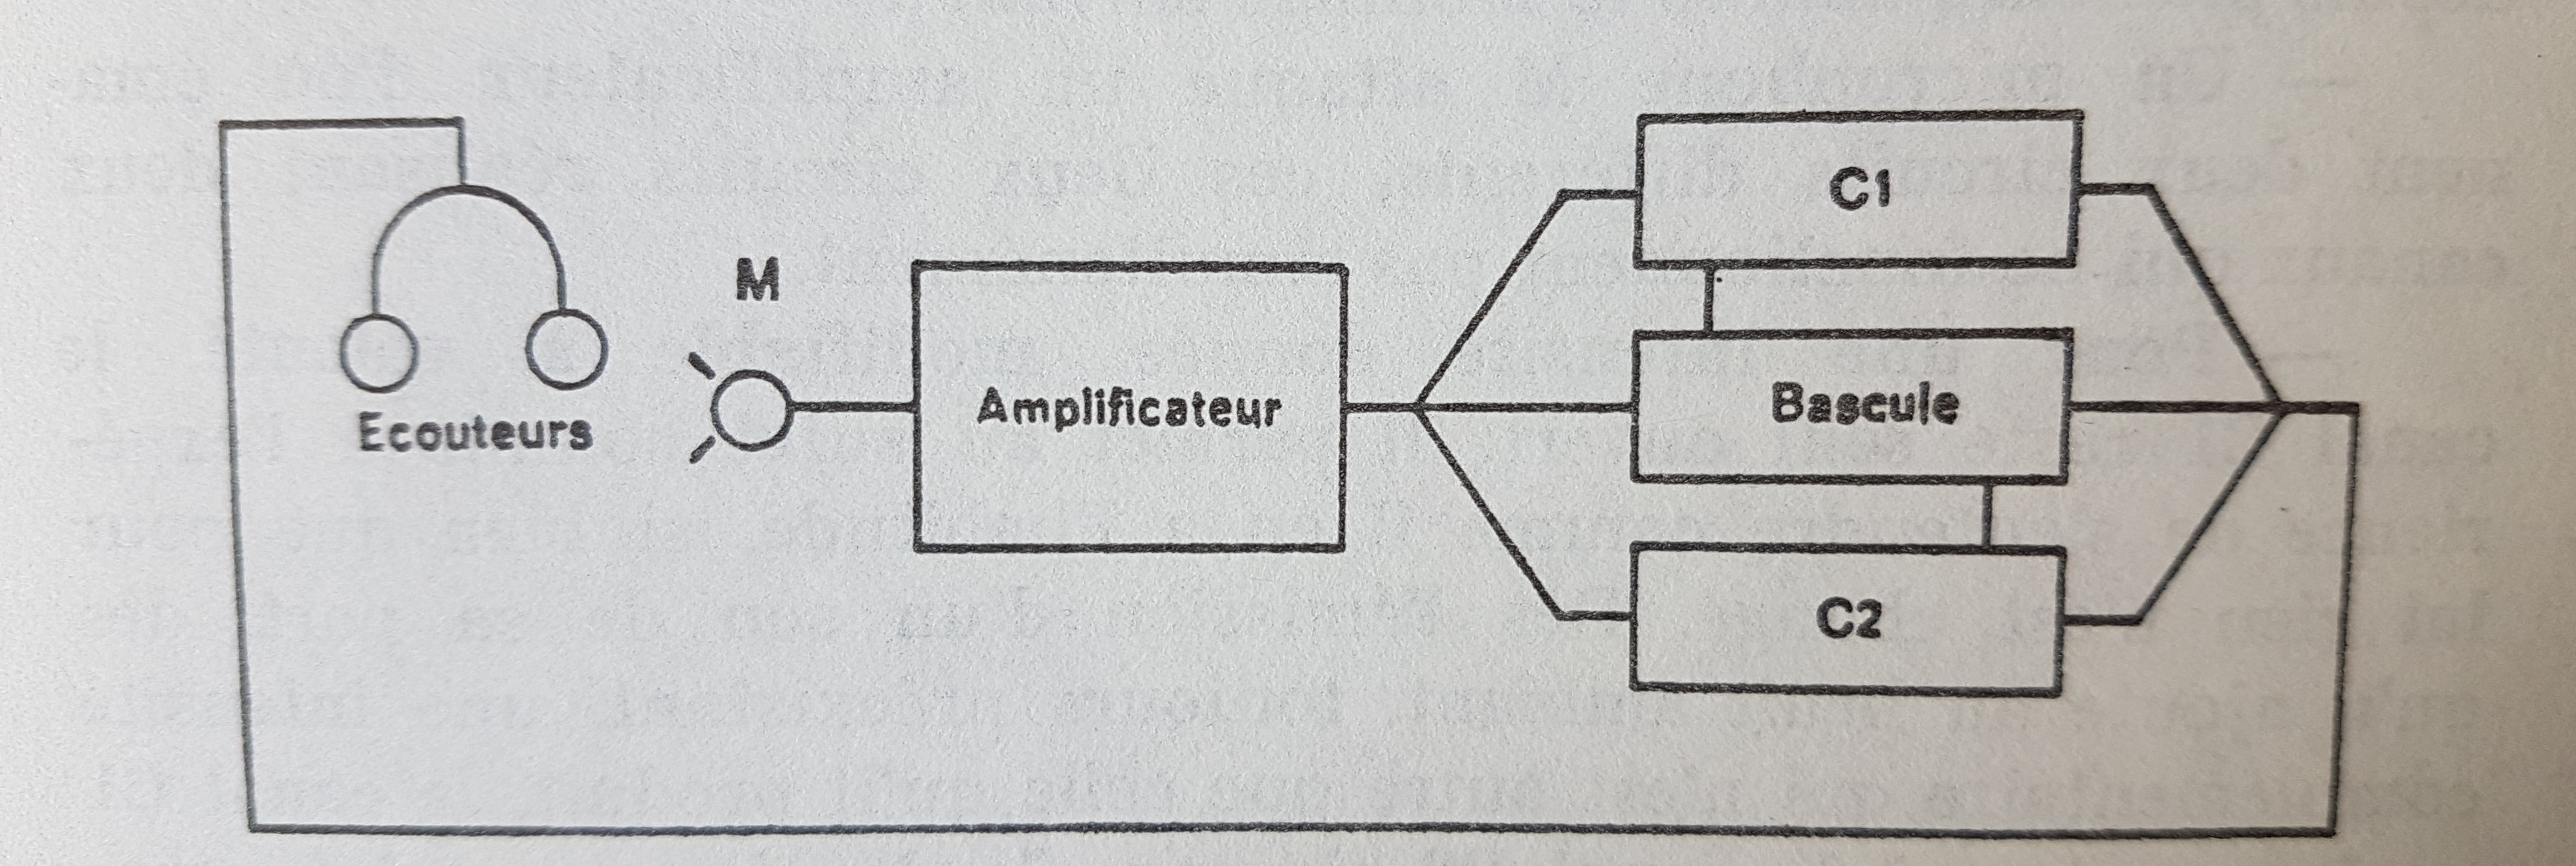
\includegraphics[width=0.7\linewidth]{images/oreilleelectro.jpg}
	\caption[oreilleelectro]{Schéma initial de l'Oreille
          Electronique}
       
	\label{oreilleelectro}
\end{figure}


      
En fait, ce schéma comprend le\textit{ feed-back}, un des principes
cybernétiques lié au concept de l'\textit{homéostasie} tel
mentonné dans le dictionnaire de psychologie.\autocite[298]{doronparot}\footnote{Doron et Parot, rétroaction;
  feedback positif = il faut varier, f.négatif= ne rien faire,  feed-back, Doron/ Parot, .p177 : cybernétique. Concept de l'homéostasie, Cannon}



 En effet, dès les premières
séances, Tomatis constate une amélioration temporaire de la voix, se
stabilisant avec l'entraînement, et établissant ainsi
\textbf{le lien frappant entre l'écoute et
  l'émission vocale}.

\textbf{L'ensemble de ces considérations préalables nous permettent d'accéder au choix de
cette méthode de testing appliquable à ma recherche.}
